\newpage
\section{Logik}
    In dem folgenden Abschnitt wird die Spiellogik bzw. die genutzten Algorithmen im Detail erläutert.
    Darunter fallen Unterprogramme zur Adressberechnung, zum Prüfen ob eine Zelle leer ist, zum Spielerwechsel,
    zum Feststellen der Länge einer Steinfolge sowie zum Feststellen des Spielendes.

    \subsection{Umrechnung der Boardadresse in eine Bufferadresse}
        Da das Spielfeld im Buffer Zeilenweise hintereinander weg verläuft, also alle 42 Zellen hintereinander liegen,
        aber auf dem Display die Zeilen untereinander angeordnet sind, müssen die Koordinaten umgerechnet werden können.
        \\
        Zum umrechnen einer Spielfeldkoordinate wird die Spaltenzahl (1 – 7) mit 8 multipliziert und mit der Zeilenzahl (1 – 6) multipliziert mit 56 addiert.
        Also bei einer Spielfeldkoordinate bei Spalte 3 und Zeile 2 währe die Berechnung folgende: (3 * 8) + (2 * 56) = 136.
        Die Multiplikatoren ergeben sich aus einer Zellenhöhe von 8 für die Zeilenzahl und aus einer Zellenbreite von 8 bei 7 Zellen pro Zeile = 56.

    \subsection{Prüfen des Zelleninhalts}
        Um Feststellen zu können ob ein Spieler eine zusammenhängende Steinfolge besitzt,
        muss es nicht nur möglich sein zu erkennen ob eine Zelle leer oder belegt ist,
        sondern ebenfalls von welchem Spieler ein Stein ist.
        \\
        Dazu wird erst im 3. Byte der Zelle (der Rand eines eventuellen Spielsteins für beide Varianten)
        geprüft ob nur Nullen (leere Zelle) oder auch Einsen (ein Spielstein von Spieler 1 oder Spieler 2) vorhanden sind.
        \\
        Wenn ein Spielstein gefunden wurde,
        wird danach geprüft ob in der Mitte des Steins Einsen vorhanden sind (ausgefüllter Spielstein) oder nicht (innen leer)
        um ihn einem Spieler zuzuordnen.

        \begin{figure}[H]
            \centering
            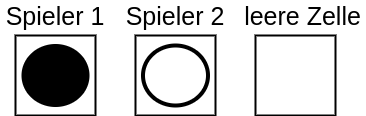
\includegraphics[scale=0.5]{img/steine.png}    
            \caption{Zellenbelegung}
        \end{figure}

    \subsection{Spielerwechsel}
        Zum Wechsel des Spielers wird der aktuelle Spieler aus der Variable „player“ ausgelesen (Spieler 1 oder Spieler 2).
        Danach wird dann auf den jeweils anderen Spieler gewechselt.

        \begin{figure}[H]
            \centering
            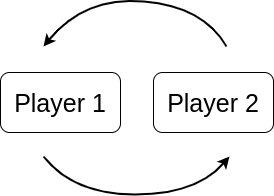
\includegraphics[scale=0.5]{img/spielerwechsel.png}    
            \caption{Spielerwechsel}
        \end{figure}


    \subsection{Feststellen der Anzahl an zusammenhängenden Steinen}
        Da der Zustand eines gewonnenen Spiels nur direkt nach dem setzen eines Steins vorkommen kann,
        wird direkt nach jedem Zug darauf geprüft.
        \\
        Um Festzustellen wie viele Steine zusammenhängend vom gleichen Spieler sind,
        werden immer von dem neu gelegten Stein zwei gegenüberliegende Seiten geprüft.
        Um die Gesamtzahl zu bestimmen muss am Ende noch eins abgezogen werden,
        damit der neu gelegte Stein nicht doppelt gezählt wird.

        \begin{figure}[H]
            \centering
            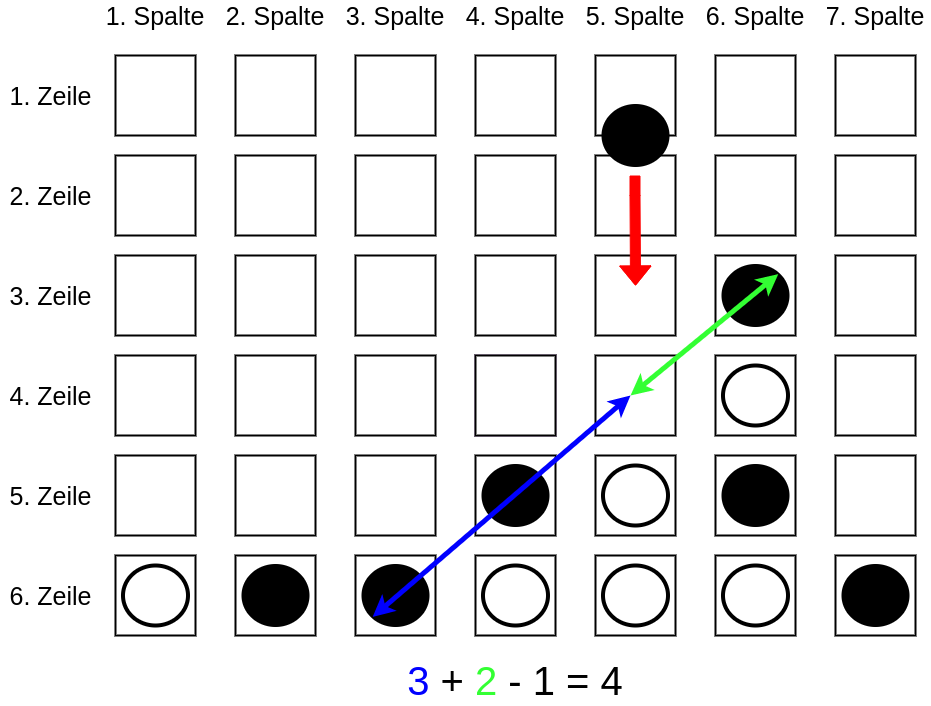
\includegraphics[scale=0.3]{img/gewinnbedingung.png}    
            \caption{Zusammenhängend Steine}
        \end{figure}

        Eine Ausnahme bilden die Richtungen oben und unten.
        Da über dem neugelegten Stein keine weiteren Steine sein können, wird nur nach unten geprüft.
        \\
        Wenn bei dem Zählen der zusammenhängenden Steine mehr als vier erkannt werden,
        bedeutet dies das Spielende und es wird die Variable \textit{playerWonFlag} auf 1 gesetzt um anschließend weitere Spielzüge zu sperren.

      